\section{Этапы Handshake}\label{COMMON.Phases}

Сеанс Handshake состоит из следующих этапов.

\begin{enumerate}
\item
Обмен ключами. Стороны согласуют параметры защиты и обмениваются ключевым 
материалом. По результатам обмена стороны формируют общие ключи, которые 
используются для защиты всех последующих сообщений.

\item
Параметры сервера. Сервер устанавливает дополнительные параметры. Например 
запрашивает аутентификацию клиента или настраивает поддержку определенных 
прикладных протоколов.

\item
Аутентификация. Проводится аутентификация сервера и, возможно, клиента. 
Аутентификация сопровождается подтверждением корректности общих ключей и 
целостности сообщений Handshake.
\end{enumerate}

% use: https://www.rfc-editor.org/errata/eid6123

На первом этапе клиент отправляет серверу приветственное 
сообщение~\token[HS.CH]{ClientHello}.
%
Сообщение содержит случайные данные клиента, перечень поддерживаемых им 
версий TLS, список поддерживаемых криптонаборов, открытые ключи протокола 
Диффи~-- Хеллмана для режима DHE и (или) набор идентификаторов секретов для 
режима PSK, другие данные.
%
Ключи и параметры для режимов DHE и PSK передаются в 
расширениях~\token[HS.Ext.ks]{key_share} и~\token[HS.Ext.psk]{pre_shared_key} 
соответственно.

Сервер обрабатывает~\token[HS.CH]{ClientHello}, выбирает параметры защиты и 
отвечает собственным приветственным сообщением~\token[HS.SH]{ServerHello}, 
в котором указывает эти параметры.
%
При использовании режима DHE сообщение~\token[HS.SH]{ServerHello} содержит
расширение~\token[HS.Ext.ks]{key_share} с открытым ключом Диффи~-- Хеллмана, 
сгенерированным сервером, а при использовании режима PSK~--- 
расширение~\token[HS.Ext.psk]{pre_shared_key} с номером секрета, выбранного 
сервером.
%
При использовании режима PSK+DHE сообщение~\token[HS.SH]{ServerHello} содержит 
оба расширения.
%
Как и клиент, сервер включает в свое приветственное сообщение случайные данные.
Наличие случайных данных обеспечивает общую волатильность сообщений Handshake 
даже при повторе всех остальных их частей.

На втором этапе сервер отправляет сообщение~\token[HS.EE]{EncryptedExtensions}.
В него включаются расширения, которые не относятся к согласованию параметров
защиты (и поэтому могут быть защищены) и не касаются сертификатов для 
аутентификации.

Если предусмотрена аутентификация клиента по сертификату, то сервер
дополнительно отправляет сообщение \token[HS.CR]{CertificateRequest}.

На третьем этапе клиент и сервер обмениваются сообщениями, которые прямо или 
косвенно поддерживают аутентификацию.

Во-первых, в сообщениях \token[HS.CT]{Certificate} стороны пересылают друг другу
свои сертификаты. Сервер не высылает сообщение \token[HS.CT]{Certificate}, если
решено использовать секрет PSK, а клиент~--- если сервер не запрашивал аутентификацию 
на основе сертификата, т.~е. не высылал сообщение \token[HS.CR]{CertificateRequest}.

Во-вторых, в сообщениях \token[HS.CV]{CertificateVerify} стороны пересылают свои
подписи стенограмм Handshake. Подпись проверяется на открытом ключе из
сертификата стороны-подписанта. Корректность подписи доказывает владение
соответствующим личным ключом и, таким образом, подлинность стороны.
%
Сообщение~\token[HS.CV]{CertificateVerify} не высылается, если аутентификация
стороны по ее сертификату не предусмотрена.

В-третьих, в сообщении \token[HS.F]{Finished} стороны обмениваются
имитовставками стенограмм Handshake. Имитовставки вычисляются на общих ключах,
сформированных на этапе~1.
%
Корректность имитовставки подтверждает знание общих ключей и, как 
следствие, владение стороной ключами, описанными в \token[HS.CH]{ClientHello} 
или \token[HS.SH]{ServerHello}.
%
При использовании режима PSK подтверждается владение предварительно 
согласованным секретом и, таким образом, подлинность стороны.

Этапы Handshake представлены на рисунке~\ref{Fig.COMMON.Phases}. Здесь и на
следующих рисунках знак ``$+$'' указывает на требующие внимания расширения,
знак ``$*$''~--- на необязательные сообщения или расширения. Фигурными
скобками окаймляются сообщения, защищенные на общих ключах для Handshake,
квадратными~--- на ключах для Record (см.~\ref{CRYPTO.Schedule}).

\begin{figure}[hbt]
\begin{center}
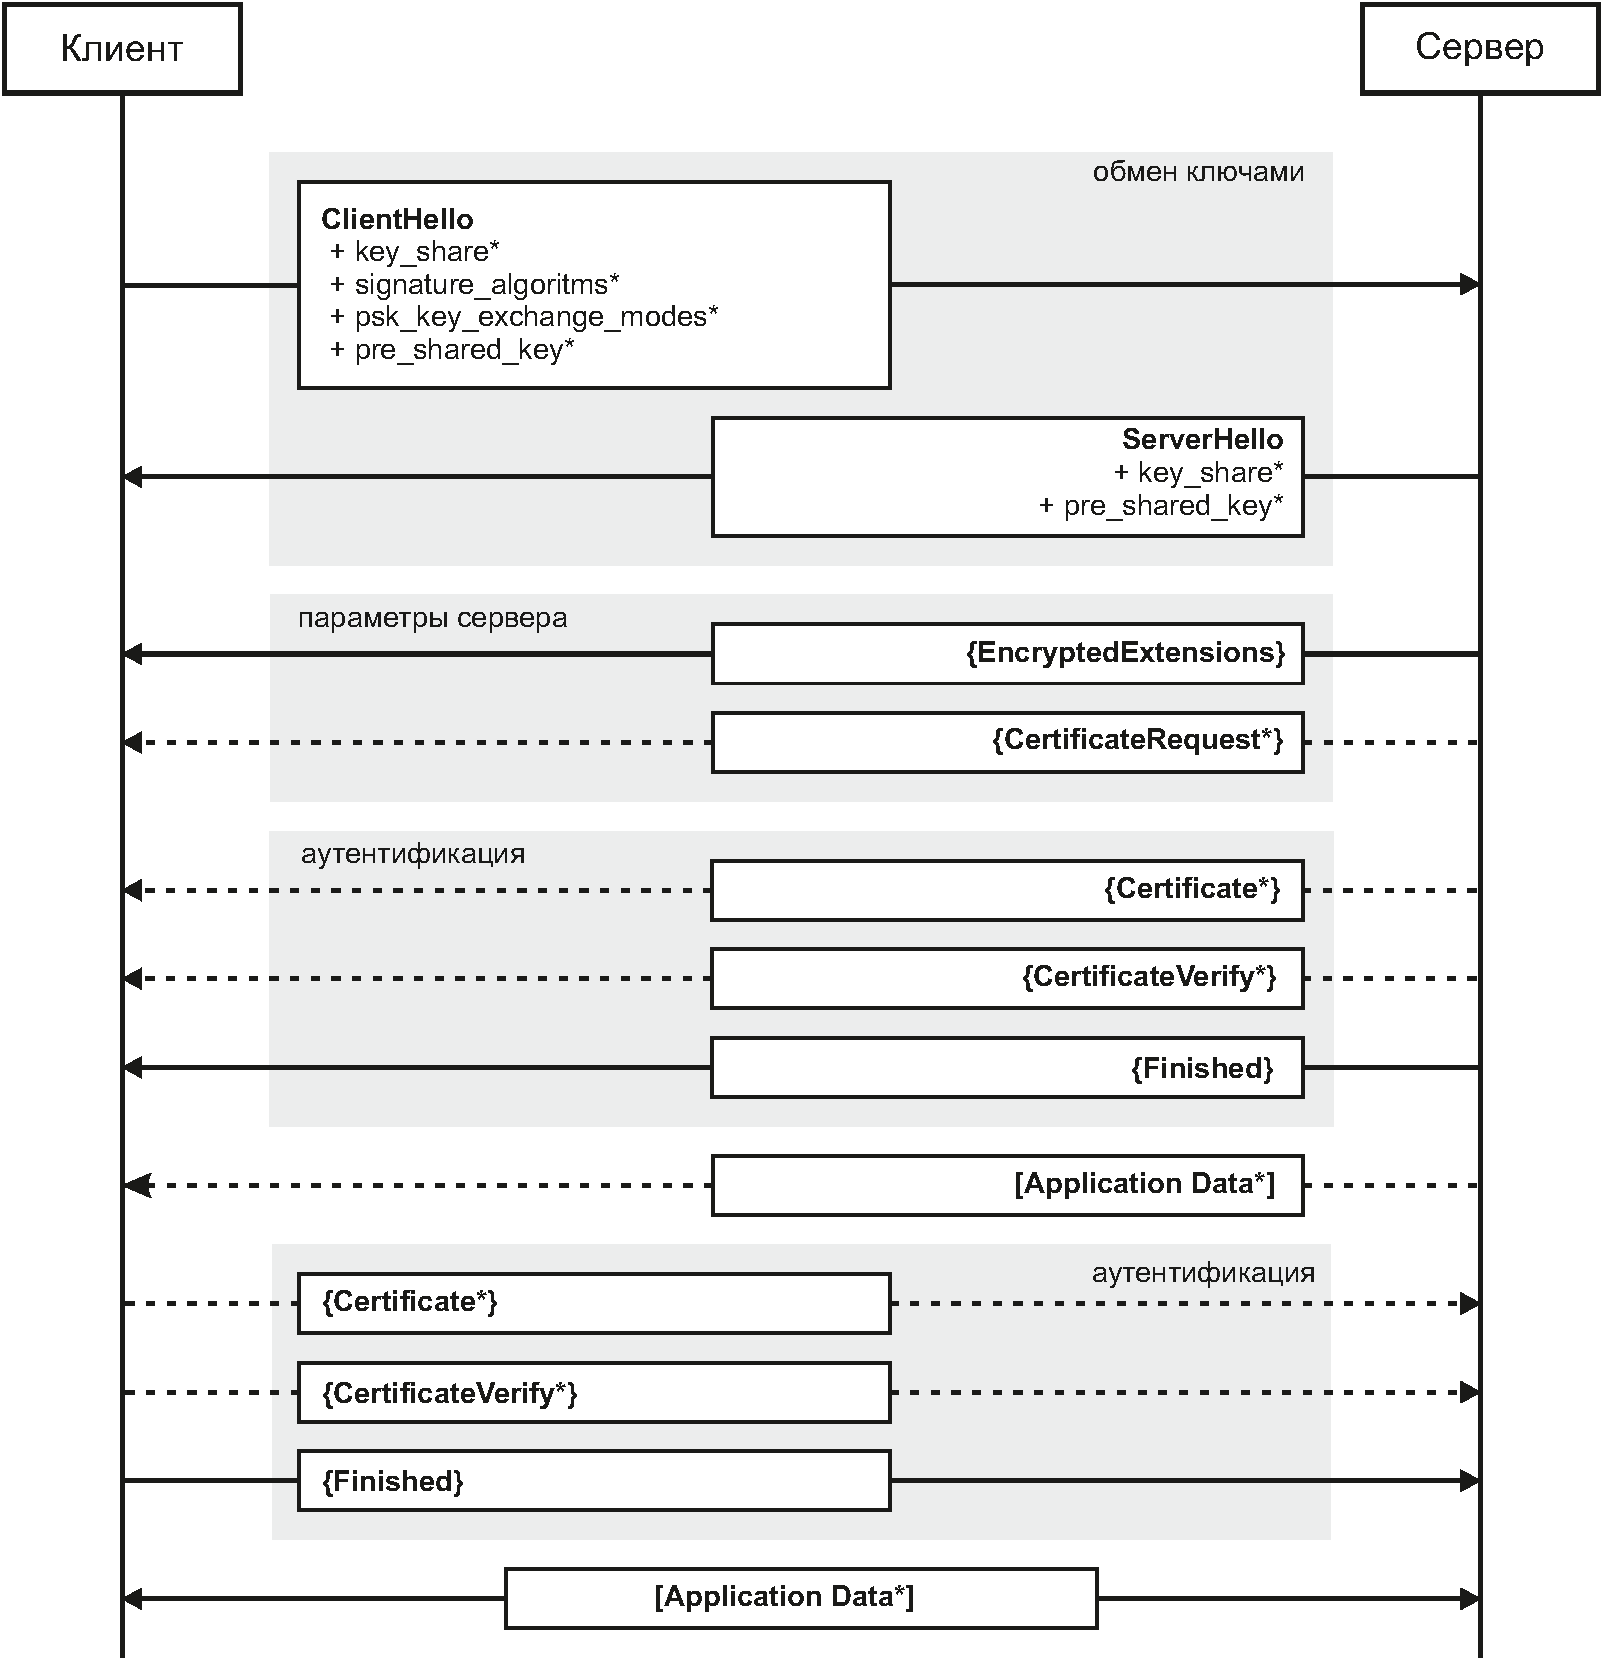
\includegraphics[width=15cm]{../figs/Phases}
\end{center}
\caption{Этапы Handshake}\label{Fig.COMMON.Phases}
\end{figure}

Отправка сообщения~\token[HS.F]{Finished} означает, что сторона завершила
Handshake и может переходить к отправке данных прикладных протоколов
(``\code{Application Data}'' на рисунке). Для ускорения работы сервер может
отправлять прикладные данные, даже не получив встречного
сообщения~\token[HS.F]{Finished} от клиента. При планировании использования TLS 
в прикладных протоколах следует учитывать, что в момент отправки сервер
взаимодействует с еще неаутентифицированным клиентом.

Еще одним способом ускорения TLS является отправка клиентом прикладных данных до
завершения Handshake, т.~е. до отправки собственного 
сообщения~\token[HS.F]{Finished}. Этот способ описан в п.~\ref{COMMON.ZeroRTT}. 

В TLS предусмотрена возможность отправки некоторых сообщений после Handshake. 
С их помощью выпускаются билеты, выполняется отложенная аутентификация, 
стороны информируют друг друга об обновлении ключей. Сообщения после Handshake 
защищаются так же, как прикладные данные.

